\chapter{Introduction}

\section{Food Combinations}
The prediction of peoples’ preferences for combinations of food items is a challenging topic that has been met with varied success.  \citet{Eindhoven1959} showed that the prediction of peoples’ preferences for combinations of food items, such as menu items, was more complex than just a linear additivity of the preference for the individual items.  The reason for this complexity is that properties such as texture, color and separation of items \citep{Eindhoven1959,Pilgrim1961}, context and consumer ethnicity \citep*{Marshall2003,Niewind1986}, frequency of consumption \citep{Marshall2003} and hypo-additivity or the “a la carte” effect \citep{Lawless1994} all contribute to our psychological models of foods.

There have been numerous attempts at specific methodologies to evaluate optimal combinations of food items.  \citet{Worsley1984} had grade school students evaluate 780 pairwise combinations of food items and answered how well “the foods in each pair would go together to form a nice meal.” This type of pairwise analysis is best analyzed by multidimensional scaling \citep{Schiffman1981}, a method of creating visual perceptual maps from similarity data. This MDS methodology has been extended by using cluster analysis to find entrées, starches and desserts that were close to each other, and followed by a regression analysis to predict compatibility ratings of the three component meal from the ratings given to the component pairs \citep{Klarman1977}.  A modified Just About Right scale \citep{Johnson1987} can also be used to evaluate optimal pairs of food items, and in the case of a wine and cheese pairing the two anchors would be “cheese dominates excessively” and “wine dominates excessively” with an “ideal match” point in the center \citep{King2005}.  \citeauthor{Niewind1986} \citep{Niewind1986} used a novel dual-scaling analysis \citep{Nishisato1984} rather than MDS to analyze pairwise similarity categories on 39 different side dishes with 4 different main items.  Dual scaling (also known as correspondence analysis or CA) provides a way of quantifying and testing for significant differences between categorical data, such as complex questionnaires.

Other strategies have evolved for evaluating more than two items, which gets at the heart of meal optimization.  Current menus can be evaluated over the course of a full menu rotation in a production setting for optimizing which overall meals provide the best hedonic scores \citep{Pagliarini2005}. Before each shuttle mission, NASA astronauts undergo tastings where they evaluate each available component (often from military Meal-Ready-To-Eat or MREs\tm and provide hedonic ratings of each \citep{Kerwin2002}.  The menus are then picked and then repeated every 4 to 6 days.  Cards with full meals listed on them can be sorted into “eat” and “not eat” piles \citep{Jonsson1991} and evaluated by proportions accepting or not accepting the full meals.

The question of how to optimize food combinations has commercial applications in restaurants and ready-to-eat home meals, and also more customized applications in institutional settings where menus are not necessarily decided on by the consumers, such as prisons and schools.

\section{Menus}
One specific type of food combination is a meal.  A meal is defined in Webster’s Revised Unabridged Dictionary as “The portion of food taken at a particular time for the satisfaction of appetite; the quantity usually taken at one time with the purpose of satisfying hunger; a repast” \citep{Webster1913}.  This definition does not capture the complexity of the meal experience and give any indication of how to control it.  The food industry has not spent much effort developing meals, rather focusing on individual items \citep{Meiselman2000}.  \citet{Meiselman2000} notes that the reason for this gap is because of the complexity of the meal experience which is composed of social, psychological \citep[see][chap. 2]{Lawless2010} and nutritional factors.  For our purposes we define a meal as a combination of foods from separate categories intended to be consumed together. 
 
An example menu for a typical southern American meal is smoked pork with barbeque sauce, corn bread, baked beans, coleslaw and lemonade.  The categories in this example are protein, sauce, starch, bread, vegetable and drink respectively.  The reason that these items work well together to create a cohesive “southern American summer barbeque” concept is beyond the scope of this paper, but it includes all of the factors listed above – social: history and tradition, psychological: flavor contrasts \citep{Lawless1977,Lawless1979,Lawless1987,Lawless2010,Lawless2000} and nutritional: protein, fat and starch.  The reader could easily come up with a favorite meal from their childhood and also note the complexity as to the reasons “why?” the favorite meal is a good concept.  
 
When consumer scientists and researchers create meals for manufacturing, it is the complexity of the meal concept that drives development, paradoxically, away from consumer driven approaches.   Many foodservice manufacturers employ research chefs or use internal “experts” to make meal concept decisions.  Other sources for concepts include teams of food scientists or established literature.  All of these approaches are notable for the lack of utilizing the intended consumer of the product as a source of information on how the components should be combined together.  

\section{Regression Approaches}
Regression analysis adds predictive capabilities to meal acceptability combination data. The regression equations typically take on some variation of this form, where meal acceptability data of the individual components predicts whole meal results \citep{Hedderley1995,Moskowitz1983,Turner1988}:

\begin{equation}
Whole Meal = \beta _{0} + \beta _1(Appetizer) + \beta _2(Entree) + \beta _3(Dessert)\
\nonumber
\end{equation}

Modifications to the regression equation have been applied to the application of cyclic menus by means of a squared coefficient \citep{Moskowitz1983} for time since last presentation.
One of the effects noted above for combinations of food items is that scores are not additive.  In one novel study individual items and meals were judged by soldiers on a barter scale, which asked them how many candy bars they would trade for a given individual food item and for combinations of food items as meals \citep{Lawless1994}. Results show that meals were discounted. When evaluated as a whole on the barter scale, the desert bars traded for the whole meal did not add up to the sum of the individual components. 
Conjoint analysis is a more advanced regression approach, based on consumer responses, which has achieved some success in predicting consumer preference \citep{Green1978,Luce1964}.  Conjoint analysis predicts combinations by presenting multiple scenarios with different factor levels of the same factor (e.g. different entrées or sauces) and finding utility scores for each factor level for its contribution to the overall concept.  Using this approach, an optimal concept can be predicted.  A more recent advancement in conjoint based approaches allows the consumers themselves to choose the factor levels in which they are interested from a list of alternatives \citep{Liechty2001}.

\section{Graph Theory}
In 1736 Leonhard Euler, a mathematician who has made great contributions to fields ranging from optics and astronomy to geometry and calculus, published a short proof known as the Kӧnigsberg Bridge Problem \citep{Euler1736}. The town of Kӧnigsberg, during the time of Euler, had seven famous bridges.  He asked whether or not a person could take a walk through the town and cross all seven bridges exactly once.  At the time it seemed like an interesting mathematician’s puzzle, but now is widely recognized as the origins of graph theory. Euler’s bridges are presented in Figure~\ref{fig:eulerbridges}, both as he drew them (left) and as a cyclic graph (right).  Using the graph, the question rephrased is simply can you draw a line such that it traverses each vertice point once and only once?  Such a path is called a Euler trail \citep{Bollobaas1998}.  Euler subsequently proved that a Euler trail was not possible using the 7 bridges.

\begin{figure}[h!]
\caption[Euler's seven bridges.]{Euler's seven bridges.  The graph on the right represents the bridge model on the left.}
\centering
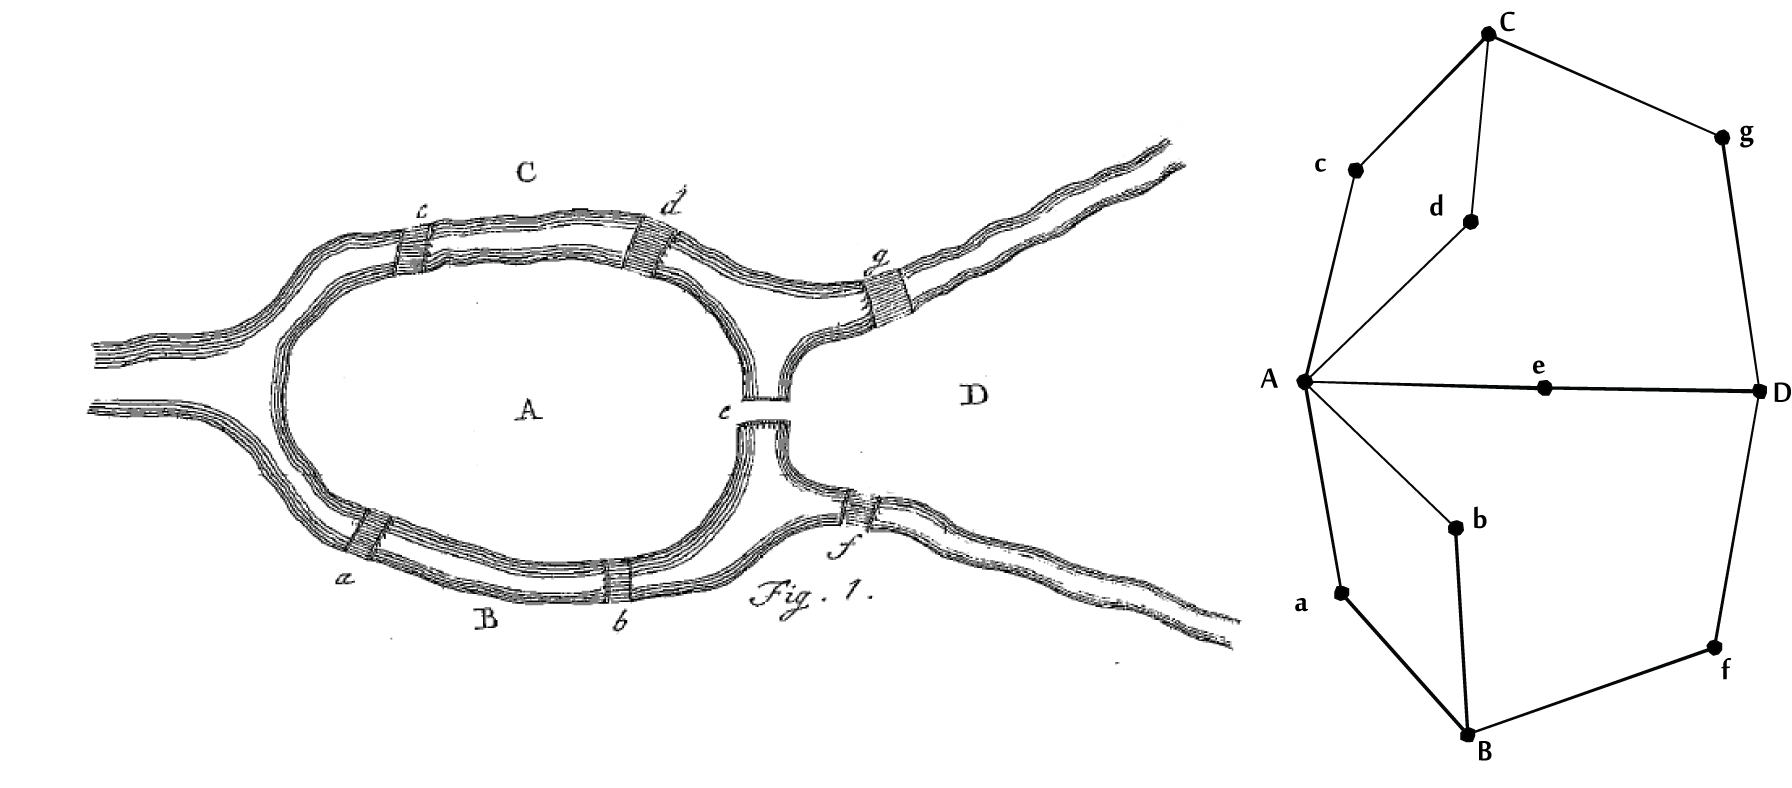
\includegraphics[width=0.9\textwidth]{./img/euler.png}
\label{fig:eulerbridges}
\end{figure}


The basic constructions of graph theory are straightforward.  A graph is a collection of objects called vertices \citep{Bollobaas1998} joined together with connections called edges.  The study of graphs is typically fruitful in any endeavor in which items may be either related or not, such as electronic circuit design \citep{Bollobaas1998},  protein interactions \citep{Palla2005}, social network analysis \citep{Knoke2008} and internet search \citep{Brin1998}.  

\section{Graph Theoretic Approach to Food Combinations}
A recent development in the search for optimal combinations of components takes a new approach, one based on relatively recent mathematical advances.  In particular, \citet{Ennisa} have proposed a graph theoretic approach to determining compatibility \citep[see also][]{Ennis2010, Ennis2011}.

To illustrate the use of graph theory in the study of food item compatibility, we view a list of 25 salad toppings as 25 vertices on a graph.  In this case, we consider vertices to be connected exactly when the salad toppings are compatible.  Our challenge of finding compatible larger collections of salad toppings can then be translated into the graph theoretic challenge of finding larger collections of vertices that are fully interconnected.  Such collections of vertices are called cliques.  In the case of subject response data, if the three pairwise combinations of ingredients Apple-Carrot, Banana-Carrot and Apple-Banana are compatible, then the larger combination or clique Apple-Banana-Carrot is a predicted compatible combination.  However, if one of the three pairs is not compatible, such as Apple-Carrot, then the larger combination is not a predicted combination (nor is it a clique).  

Using this clique finding technique, vast numbers of combinations can be eliminated from consideration, allowing the researcher to focus attention on a short of list of fully compatible combinations.  This method is not meant to supplant existing techniques but rather is meant to complement existing methods by helping researchers screen large numbers of combinations down to a reasonable size list that can then be analyzed in greater detail.  

\section{Research Program}
The goal of the current research program is to apply the \citet{Ennisa} graph theoretic approach to foods and to propose an extension to the approach for menus and to test the validity of a crucial assumption.  In particular, in any product category in which we wish to apply the graph theoretic approach, in order to justify the elimination of combinations that are not fully pairwise compatible and to reasonably focus only on combinations that are fully pairwise compatible (i.e. the cliques), we need to know that the following assumption holds:

\noindent
{\bf Principle of Supercombinatorality (SC):} Combinations that are fully pairwise compatible will be considered more compatible overall than combinations that are not fully pairwise compatible.

SC is so named as it asserts that compatible combinations can be super-constructed from compatible pairs.  In the language of food science, SC says that compatible food products can be constructed from compatible food components.  In the language of graph theory, SC says that cliques will be considered more compatible than non-cliques.
In doing so, we will validate the underlying psychological effect, the property of supercombinatorality, which allows us to take pairwise consumer response data and scale it up to larger combinations.  This novel approach is then extended to menu development where cross category comparisons are introduced and an analysis is proposed.  Finally, we show a method for ranking the results to provide more specific feedback to consumer scientists.  

\pagebreak
\renewcommand\bibname{{REFERENCES}} %  will print "REFERENCES" instead of "BIBLIOGRAPHY"
\phantomsection
\addcontentsline{toc}{section}{References} %  adds "REFERENCES" to the table of content
\bibliographystyle{apalike}
\bibliography{library_man}  % uses the references stored in Chapter1Radar.bib